\chapter{ما يحتاج إليه النبات}\label{ch:g4:what-plants-need}

أصيصان من الرشاد على حافة النافذة نفسها، بُذرا في اليوم نفسه.
يُسقى أحدهما ولا يُسقى الآخر --- وفي غضون أسبوع يُكتب الفرق باللون
الأخضر واللون الأصفر. وبأصص \omterm{def:g2:from-seed-to-plant:seed}{وبذور} وصبر تستطيع أن تجعل \omterm{def:g1:plants-around-us:plant}{النباتات}
نفسها تجيب عن سؤال هذا الفصل: ما الذي يحتاج إليه \omterm{def:g1:plants-around-us:plant}{النبات} بالضبط
ليعيش وينمو؟

\section{سؤال النباتات: الاختبار المنصف}

\begin{method}[الاختبار المنصف]\label{met:g4:what-plants-need:fairtest}
لتعرف أيحتاج \omterm{def:g1:plants-around-us:plant}{النبات} إلى شيء ما --- ماء، أو ضوء، أو تربة، أو دفء:
\begin{enumerate}
  \item خذ \emph{أصيصين} من \omterm{def:g1:plants-around-us:plant}{النباتات} نفسها، مبذورين بالطريقة
        نفسها؛
  \item وعاملهما معاملة واحدة في كل شيء \emph{إلا الشيء الواحد
        المختبَر} --- فينال أحدهما إياه ولا يناله الآخر؛
  \item وانتظر أيامًا أو أسابيع، ثم قارن؛
  \item وكل فرق لا بد أن يأتي من الشيء الواحد الذي غيّرته: فقد
        كان الاختبار منصفًا.
\end{enumerate}
ويسمى الأصيص الذي لم يُمسّ \emph{الشاهد}\index{شاهد (تجربة)}: فهو
يبين ما يحدث حين لا ينقص شيء.
\end{method}

\begin{example}[لماذا أصيصان لا أصيص واحد]\label{ex:g4:what-plants-need:control}
لنفترض أن أصيصًا واحدًا غير مسقيّ ذبل. أفكان ذلك من نقص الماء ---
أم من موجة برد، أم من \omterm{def:g2:from-seed-to-plant:seed}{بذور} رديئة؟ فإذا وقف بجانبه توأمه المسقيّ
أخضر، وقد نبتا من الكيس نفسه في الغرفة نفسها، زال الشك: فالتوأمان
لم يختلفا إلا في الماء. وتجارب الأصيص الواحد لا تقنع أحدًا، ولا
سيما عالم أحياء.
\end{example}


\begin{omfigure}
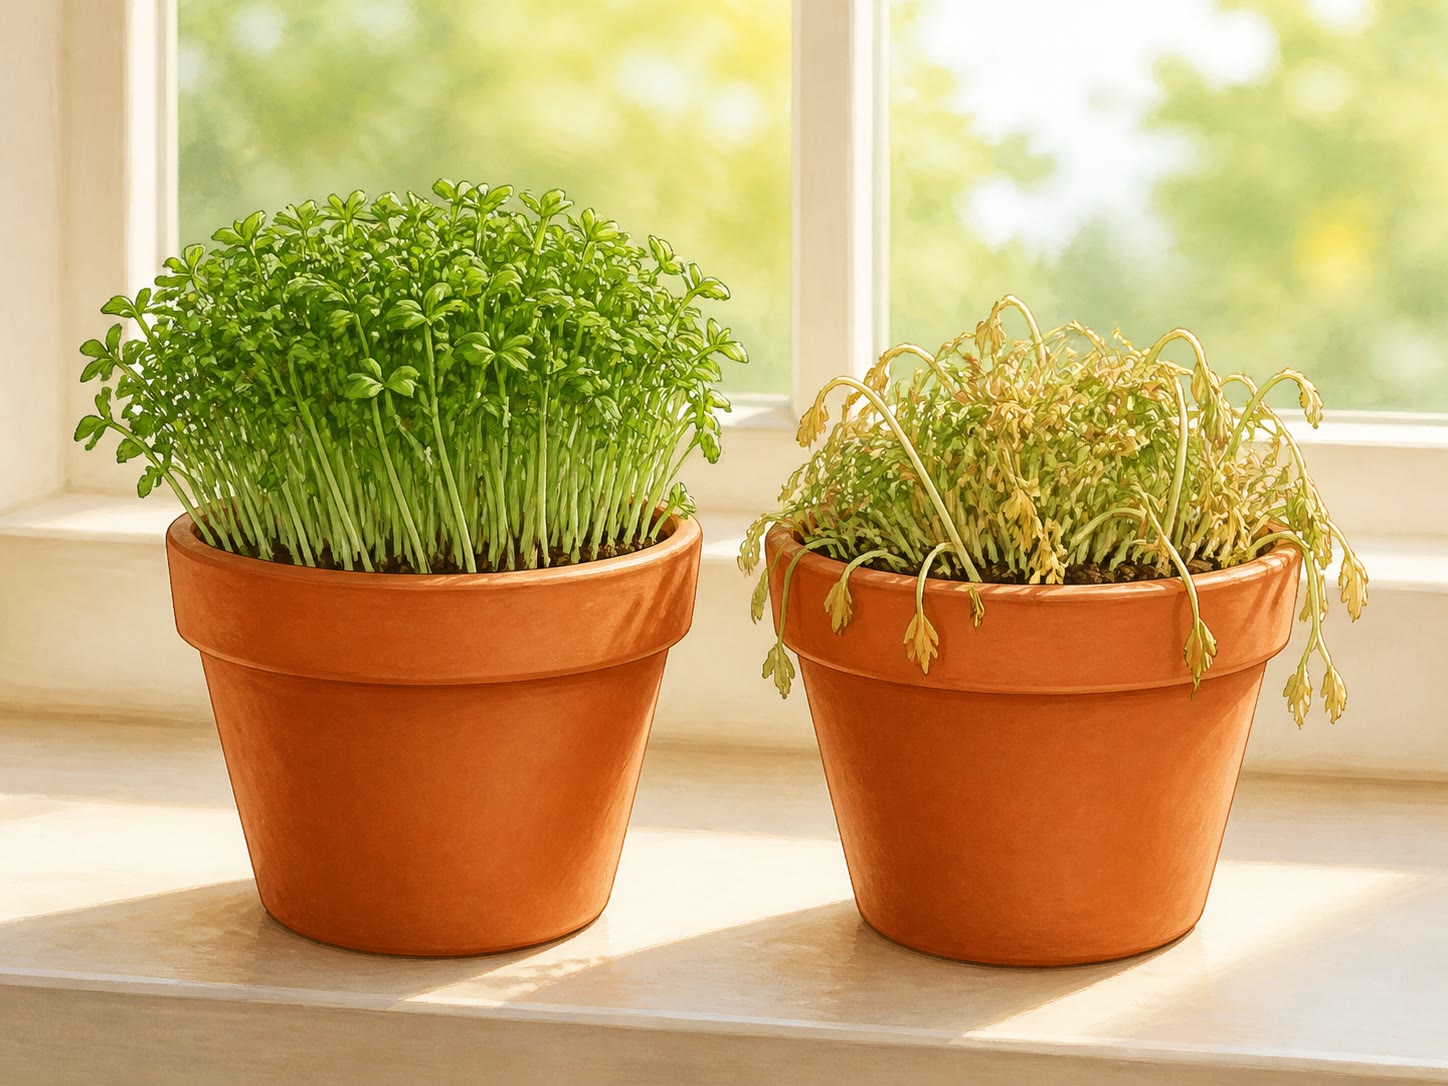
\includegraphics[width=0.58\linewidth]{images/book1/ai/g4-plants-cresspots.jpg}

{\small التجربة نفسها على حافة نافذة حقيقية، بعد أسبوع: التوأمان
يختلفان الآن في كل ما يُرى --- لأنهما اختلفا في شيء واحد فحسب.}
\end{omfigure}

\section{ما تكشفه الاختبارات}

\begin{proposition}[حاجات النبات]\label{prop:g4:what-plants-need:needs}
تبين الاختبارات المنصفة، مُجراةً لكل حاجة على حدة، أن \omterm{def:g1:plants-around-us:plant}{النبات} يحتاج إلى:
\begin{itemize}
  \item \emph{الماء} --- فالأصيص غير المسقيّ يذبل ويموت؛
  \item و\emph{الضوء} --- فأصيص الخزانة ينمو شاحبًا طويلًا ضعيفًا
        ثم يستسلم: فلا ضوء، ولا غذاء نباتيًّا مصنوعًا؛
  \item و\emph{الهواء} --- فإذا عُزل عن الهواء الطلق توقف النمو؛
  \item و\emph{الدفء} --- ففي البرد تنتظر \omterm{def:g2:from-seed-to-plant:seed}{البذور}
        (\cref{prop:g2:from-seed-to-plant:needs}) ويتجمد النمو حتى
        يقف؛
  \item و\emph{الأملاح المعدنية}\index{أملاح معدنية}: وهي مقادير
        ضئيلة من مواد مغذية تشربها \omterm{def:g1:plants-around-us:parts}{الجذور} مذابة في ماء التربة ---
        وفي الماء النقي وحده يعوز \omterm{def:g1:plants-around-us:plant}{النبات} سريعًا.
\end{itemize}
\end{proposition}
\admitted

\begin{example}[السجين الشاحب]\label{ex:g4:what-plants-need:pale}
اختبار الخزانة في \cref{exo:g1:plants-around-us:8}، إذا أُجري
كما ينبغي مع توأم مضاء، يعطي نتيجة لافتة: فالسجين ليس حزينًا
فحسب بل \emph{أصفر شاحب} --- إذ كفّ عن صنع مادته الخضراء ---
و\emph{طويل} على نحو غريب، ممتدّ كأنه يبحث عن الضوء الغائب. والنمو
بلا ضوء إنفاق بلا كسب؛ فإذا احترقت مدخرات \omterm{def:g2:from-seed-to-plant:seed}{البذرة} توقف.
\end{example}

\begin{remark}[لماذا يغذّي البستانيون التربة]\label{rem:g4:what-plants-need:soil}
السماد والروث ليسا ``وجبات'' \omterm{def:g1:plants-around-us:plant}{للنبات} --- \omterm{def:g1:plants-around-us:plant}{فالنباتات} لا تأكل أحدًا.
بل هما يعيدان تموين أملاح التربة المعدنية التي تحملها المحاصيل
بعيدًا سنة بعد سنة. وصندوق السماد في
\cref{ex:g2:caring-for-nature:compost} يغلق الحلقة: فما أعطته
التربة للخضر، تردّه القشور إلى التربة.
\end{remark}

\section{ماذا تفعل النباتات بما تأخذه}

\begin{proposition}[النباتات تصنع مادتها بنفسها]\label{prop:g4:what-plants-need:make}
\omterm{def:g1:animals-around-us:animal}{الحيوانات} تنمو بأكل كائنات حية أخرى. أما \omterm{def:g1:plants-around-us:plant}{النبات} فلا يأكل أحدًا:
فبالماء \omterm{prop:g4:what-plants-need:needs}{والأملاح المعدنية} من التربة، وبالهواء، وبطاقة \emph{الضوء}
التي تلتقطها أوراقه الخضراء، \emph{يصنع مادته بنفسه} --- سيقانًا
وأوراقًا وجذورًا وبذورًا جديدة. ولهذا كان الضوء أمرًا جدّيًّا يقوم عند
\omterm{def:g1:plants-around-us:plant}{النبات} مقام الطعام والشراب، ولهذا تواجه \omterm{def:g1:plants-around-us:parts}{الورقة} الخضراء السماء.
\end{proposition}
\admitted

\begin{example}[شجرة من لا شيء تقريبًا]\label{ex:g4:what-plants-need:tree}
ازرع \omterm{def:g2:from-seed-to-plant:seed}{بذرة} في أصيص كبير من تربة موزونة، وانتظر سنوات، فإذا شجرة
صغيرة قائمة هناك --- ومع ذلك لم تفقد التربة شيئًا من وزنها
تقريبًا. فخشب الشجرة لم يُغرف من الأصيص: بل \emph{صُنع}، من الماء
والهواء والضوء، في مشاغل \omterm{def:g1:plants-around-us:parts}{الأوراق} الخضراء. ومن أين تأتي مادة
الكائنات الحية سؤال سيشغلنا من جديد في سنوات لاحقة.
\end{example}

\begin{remark}[الأخضر يكسب قوت الجميع]\label{rem:g4:what-plants-need:everyone}
تذكّر \cref{prop:g3:food-chains:start}: كل \omterm{def:g3:food-chains:chain}{سلسلة غذائية} تبدأ
\omterm{def:g1:plants-around-us:plant}{بنبات}. والآن نرى لماذا وجب ذلك --- \omterm{def:g1:plants-around-us:plant}{فالنباتات} هي الحلقة الوحيدة
التي تصنع مادة جديدة من مكوّنات غير حية. وكل لقمة يأكلها أحد، في
أي مكان، صُنعت في \omterm{def:g1:plants-around-us:parts}{ورقة} أولًا.
\end{remark}

\section{تمارين}

\begin{exercise}[$\star$]\label{exo:g4:what-plants-need:1}
عدّد حاجات \omterm{def:g1:plants-around-us:plant}{النبات} الخمس.
\end{exercise}

\begin{exercise}[$\star$]\label{exo:g4:what-plants-need:2}
في الاختبار المنصف، كم شيئًا يجوز أن يختلف بين الأصيصين؟ وما اسم
الأصيص الذي لم يُمسّ؟
\end{exercise}

\begin{exercise}[$\star$]\label{exo:g4:what-plants-need:3}
صف مظهر \omterm{def:g1:plants-around-us:plant}{نبتة} نمت أسبوعين في الظلام. وأي حاجة كانت ناقصة، وما الذي
لم تستطع صنعه؟
\end{exercise}

\begin{exercise}[$\star$]\label{exo:g4:what-plants-need:4}
ما \omterm{prop:g4:what-plants-need:needs}{الأملاح المعدنية}، وكيف يأخذها \omterm{def:g1:plants-around-us:plant}{النبات}؟
\end{exercise}

\begin{exercise}[$\star$]\label{exo:g4:what-plants-need:5}
لماذا ينثر البستانيون السماد، \omterm{def:g1:plants-around-us:plant}{والنباتات} لا تأكل؟
\end{exercise}

\begin{exercise}[$\star$]\label{exo:g4:what-plants-need:6}
بم تختلف طريقة نمو \omterm{def:g1:plants-around-us:plant}{النبات} عن طريقة نمو \omterm{def:g1:animals-around-us:animal}{الحيوان}، وفق
\cref{prop:g4:what-plants-need:make}؟
\end{exercise}

\begin{exercise}[$\star$]\label{exo:g4:what-plants-need:7}
في \cref{ex:g4:what-plants-need:tree}، لم تكد تربة الأصيص تفقد
وزنًا بينما نمت الشجرة. فمن أين جاءت مادة الشجرة؟
\end{exercise}

\begin{exercise}[$\star$]\label{exo:g4:what-plants-need:8}
جرّب: صمّم اختبار الماء المنصف في الشكل وأجره على الرشاد ---
أصيصان، وفرق واحد. وسجّل ما ترى بعد أسبوع.
\end{exercise}

\begin{exercise}[$\star\star$]\label{exo:g4:what-plants-need:9}
``يبرهن'' لوكاس على أن \omterm{def:g1:plants-around-us:plant}{النباتات} تحتاج إلى الموسيقى: فقد غنّى
لأصيص واحد شهرًا فازدهر. فما الذي ينقص تجربته وفق
\cref{met:g4:what-plants-need:fairtest}؟ صمّم النسخة التي تختبر
ذلك فعلًا.
\end{exercise}

\begin{exercise}[$\star\star$]\label{exo:g4:what-plants-need:10}
\omterm{def:g1:plants-around-us:plant}{نبتة} مائية تنمو مغمورة كليًّا، بلا \omterm{def:g1:plants-around-us:parts}{جذور}، وهي صحيحة مع ذلك. فأي
حاجة من الحاجات الخمس ما زالت تلبّيها بوضوح، وكيف --- وأي حاجة
يوفّرها لها ماؤها مكان التربة؟
\end{exercise}

\begin{exercise}[$\star\star\star$]\label{exo:g4:what-plants-need:11}
أصيصان متطابقان من النعناع: أحدهما في رمل بماء مطر نقي، والآخر في
تربة حديقة، وكلاهما مسقيّ ومضاء بالتساوي. وبعد شهرين يكون أصيص
الرمل صغيرًا مصفرًّا. فأي حاجة يعزلها هذا الاختبار المنصف --- ولماذا
نمت \omterm{def:g1:plants-around-us:plant}{نبتة} الرمل أصلًا في البداية؟
\end{exercise}
